We implemented our method
and compared it with the older ones.
The results are very promising.

Figure \ref{fig:results} shows our results:
Figure \ref{fig:results}(a) gives a scatter-plot
of the $N$ sound-clips, where the axis are the two main
features we propose to use $\ldots$
Figure \ref{fig:results}(b) shows the wall-clock time
of our method, versus the size of the database $N$.

\begin{figure}[htbf]
\begin{center}
\begin{tabular}{cc}
     % uncomment the next lines, and give the right ps files
     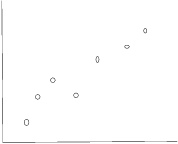
\includegraphics[width=0.3\textwidth]{FIG/data.png} &
     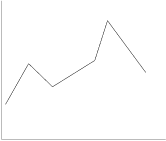
\includegraphics[width=0.3\textwidth]{FIG/plot.png} \\
     %\psfig{figure=FIG/plot.ps,width=2in} \\
     % \psfig{figure=FIG/data.ps,width=2in} &
     % \psfig{figure=FIG/plot.ps,width=2in} \\
    (a) & (b) 
\end{tabular}
\caption{A fictitious dataset (a) and its performance plot (b)}
\label{fig:results}
\end{center}
\end{figure}

